% Appendix C

\chapter{Resultados Detalhados da Validação LOSO Polar H10}
\label{AppendixC}

\counterwithin{table}{subsection}
\counterwithin{figure}{subsection}
\renewcommand{\thetable}{\thesubsection}
\renewcommand{\thefigure}{\thesubsection}

Este apêndice apresenta os resultados detalhados da validação \textit{Leave-One-Subject-Out} (LOSO) dos modelos de classificação XGBoost, Random Forest, SVM e Regressão Logística. Incluem-se as tabelas de desempenho por trabalhador, os \textit{Classification Reports} por classe e as matrizes de confusão individuais e agregadas, permitindo analisar de forma detalhada o desempenho de cada modelo.

\section{Resultados: Modelo Random Forest}

Os resultados seguintes apresentam o desempenho do modelo Random Forest na validação LOSO com dados do Polar H10. A análise inclui a Tabela~\ref{tab:loso_random_forest_detalhado}, que apresenta o desempenho por trabalhador, a Tabela~\ref{tab:classification_report_random_forest}, correspondente ao relatório de classificação por classe, e a Tabela~\ref{tab:matriz_confusao_agregada_random_forest}, que apresenta a matriz de confusão agregada dos dez folds. A Figura~\ref{fig:confusao_random_forest} apresenta as matrizes de confusão individuais para cada trabalhador utilizado como conjunto de teste.

\subsection{Tabela de desempenho da validação LOSO}

A tabela apresenta, para cada trabalhador utilizado como teste, o conjunto de trabalhadores utilizado no treino e as principais métricas de avaliação do modelo.

\begin{table}[H]
\centering
\caption{Validação LOSO do modelo Random Forest.}
\label{tab:loso_random_forest_detalhado}
\tiny
\resizebox{\textwidth}{!}{%
\begin{tabular}{l l r r r r r r}
\hline
\textbf{Teste} & \textbf{Treino} & \textbf{Recall LOW} & \textbf{Recall MED} & \textbf{Recall HIGH} & \textbf{Accuracy} & \textbf{Balanced Accuracy} & \textbf{Macro-F1} \\
\hline
W00 & W01--W09 & 0,952381 & 0,500000 & 0,642857 & 0,884615 & 0,698413 & 0,701451 \\
W01 & W00, W02--W09 & 0,980583 & 0,818898 & 0,982143 & 0,916797 & 0,927208 & 0,907259 \\
W02 & W00--W01, W03--W09 & 0,883721 & 0,841727 & 0,912134 & 0,875622 & 0,879194 & 0,852795 \\
W03 & W00--W02, W04--W09 & 0,876923 & 0,680000 & 0,990536 & 0,953317 & 0,849153 & 0,860202 \\
W04 & W00--W03, W05--W09 & 0,968421 & 0,784810 & 1,000000 & 0,943060 & 0,917744 & 0,844123 \\
W05 & W00--W04, W06--W09 & 0,952381 & 0,937500 & 0,904762 & 0,932432 & 0,931548 & 0,934436 \\
W06 & W00--W05, W07--W09 & 1,000000 & 0,666667 & 1,000000 & 0,942857 & 0,888889 & 0,917460 \\
W07 & W00--W06, W08--W09 & 1,000000 & 0,312500 & 0,860465 & 0,746269 & 0,724322 & 0,642868 \\
W08 & W00--W07, W09 & 0,385542 & 0,465116 & 0,571429 & 0,421053 & 0,474029 & 0,378676 \\
W09 & W00--W08 & 1,000000 & 1,000000 & 1,000000 & 1,000000 & 1,000000 & 1,000000 \\
\hline
\textbf{Média} & \textit{Média dos folds} & 0,899995 & 0,700722 & 0,886433 & 0,861602 & 0,829050 & 0,803927 \\
\hline
\end{tabular}%
}
\end{table}

\subsection{Relatório de classificação por classe}

O relatório de classificação por classe apresenta o \textit{support}, o \textit{recall} e a \textit{precision} obtidos para as categorias LOW, MED e HIGH na avaliação LOSO.

\begin{table}[H]
\centering
\caption{Relatório de Classificação por Classe (Classification Report) do modelo Random Forest na avaliação LOSO.}
\label{tab:classification_report_random_forest}
\begin{tabular}{l c c c}
\hline
\textbf{Classe} & \textbf{Support} & \textbf{Recall} & \textbf{Precision} \\
\hline
Low & 950 & 0,904 & 0,897 \\
Medium & 744 & 0,790 & 0,824 \\
High & 944 & 0,952 & 0,931 \\
\hline
\end{tabular}
\end{table}

\subsection{Matriz de confusão agregada}

A matriz de confusão agregada reúne as previsões dos dez folds. As linhas representam as classes reais e as colunas representam as classes previstas pelo modelo.

\begin{table}[H]
\centering
\caption{Matriz de Confusão Agregada dos Dez Folds do Random Forest na avaliação LOSO.}
\label{tab:matriz_confusao_agregada_random_forest}
\begin{tabular}{l c c c}
\hline
 & \textbf{Low} & \textbf{Medium} & \textbf{High} \\
\hline
\textbf{Low} & 859 & 83 & 8 \\
\textbf{Medium} & 97 & 588 & 59 \\
\textbf{High} & 2 & 43 & 899 \\
\hline
\end{tabular}
\end{table}

\clearpage
\subsection{Matrizes de confusão por trabalhador}

A figura apresenta as matrizes de confusão individuais obtidas para cada trabalhador utilizado como conjunto de teste.

\begin{center}
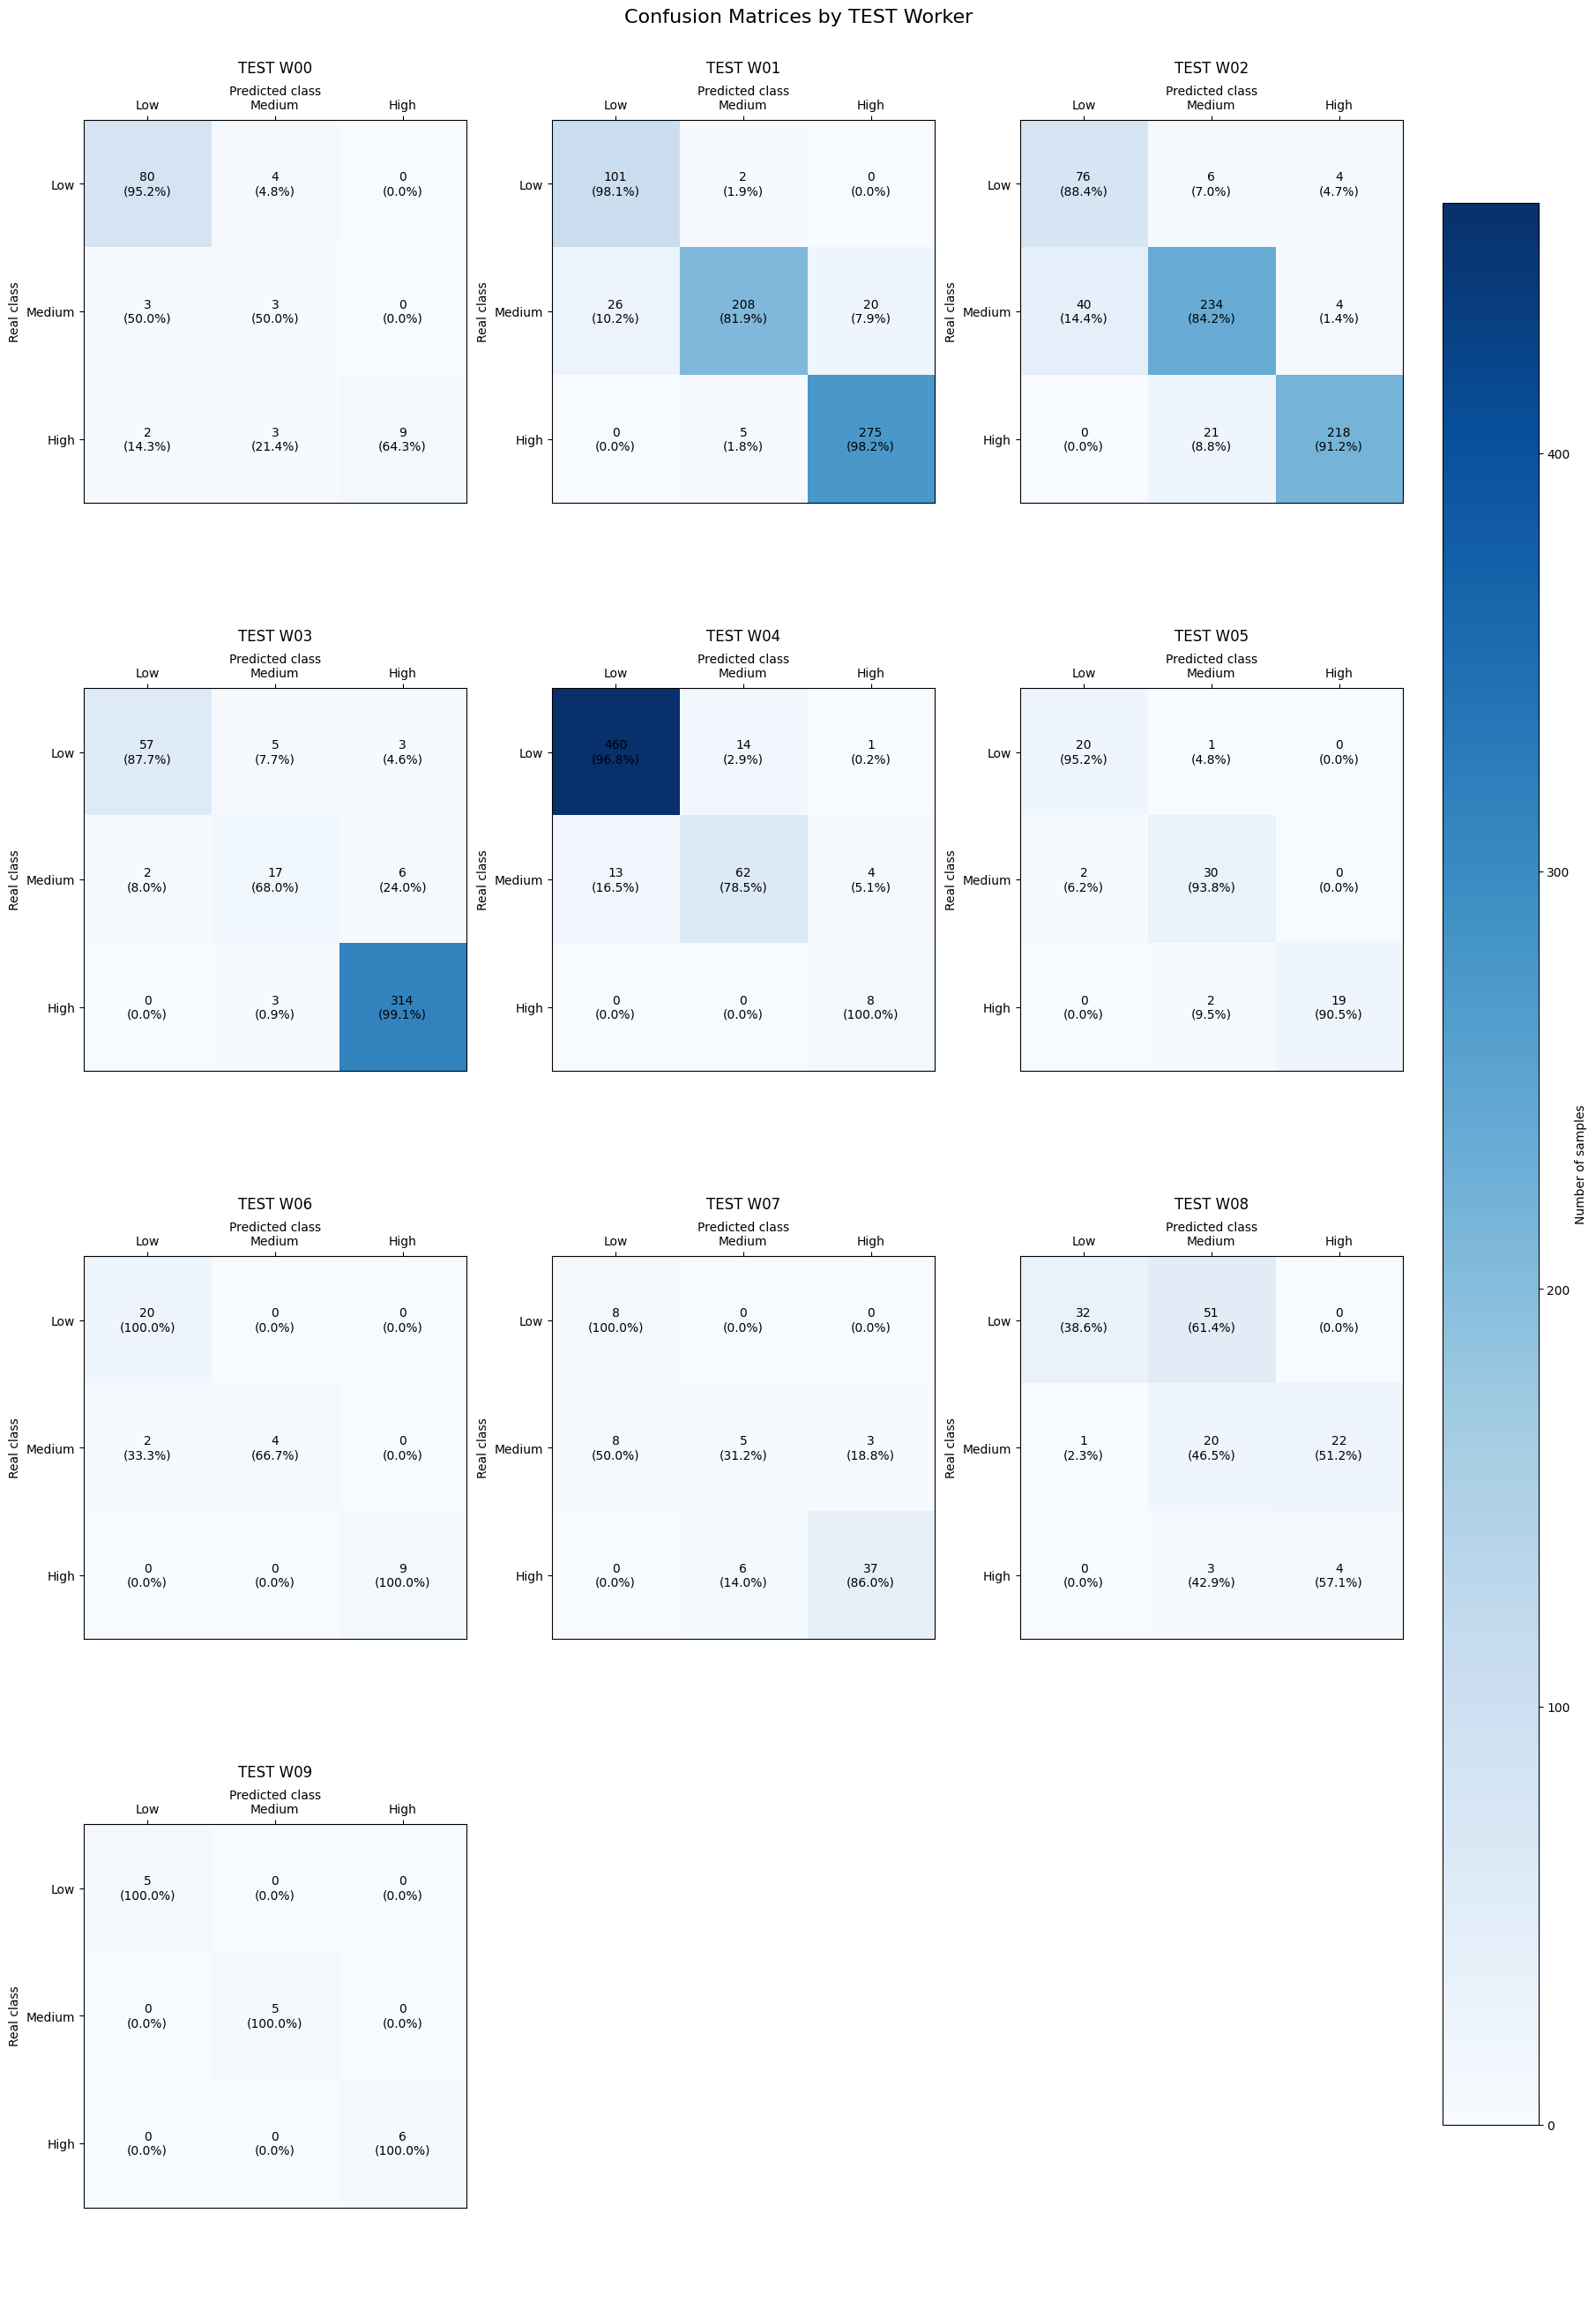
\includegraphics[width=\textwidth,height=\dimexpr\textheight-\pagetotal-4\baselineskip\relax,keepaspectratio]{ch4/assets/confusionrandomforest..png}
\captionof{figure}{Matrizes de confusão do Random Forest por trabalhador de teste.}
\label{fig:confusao_random_forest}
\end{center}

\section{Resultados: Modelo SVM}

Os resultados seguintes apresentam o desempenho do modelo SVM na validação LOSO com dados do Polar H10. A análise inclui a Tabela~\ref{tab:loso_svm_detalhado}, que apresenta o desempenho por trabalhador, a Tabela~\ref{tab:classification_report_svm}, correspondente ao relatório de classificação por classe, e a Tabela~\ref{tab:matriz_confusao_agregada_svm}, que apresenta a matriz de confusão agregada dos dez folds. A Figura~\ref{fig:confusao_svm} apresenta as matrizes de confusão individuais para cada trabalhador utilizado como conjunto de teste.

\subsection{Tabela de desempenho da validação LOSO}

A tabela apresenta, para cada trabalhador utilizado como teste, o conjunto de trabalhadores utilizado no treino e as principais métricas de avaliação do modelo.

\begin{table}[H]
\centering
\caption{Validação LOSO do modelo SVM.}
\label{tab:loso_svm_detalhado}
\tiny
\resizebox{\textwidth}{!}{%
\begin{tabular}{l l r r r r r r}
\hline
\textbf{Teste} & \textbf{Treino} & \textbf{Recall LOW} & \textbf{Recall MED} & \textbf{Recall HIGH} & \textbf{Accuracy} & \textbf{Balanced Accuracy} & \textbf{Macro-F1} \\
\hline
W00 & W01--W09 & 0,952381 & 0,666667 & 0,785714 & 0,913462 & 0,801587 & 0,762146 \\
W01 & W00, W02--W09 & 0,883495 & 0,862205 & 0,875000 & 0,871272 & 0,873567 & 0,858319 \\
W02 & W00--W01, W03--W09 & 0,813953 & 0,816547 & 0,979079 & 0,880597 & 0,869860 & 0,855888 \\
W03 & W00--W02, W04--W09 & 0,907692 & 0,600000 & 0,933754 & 0,909091 & 0,813815 & 0,766801 \\
W04 & W00--W03, W05--W09 & 0,957895 & 0,886076 & 0,750000 & 0,944840 & 0,864657 & 0,761599 \\
W05 & W00--W04, W06--W09 & 0,857143 & 0,843750 & 0,857143 & 0,851351 & 0,852679 & 0,855993 \\
W06 & W00--W05, W07--W09 & 0,850000 & 0,166667 & 1,000000 & 0,771429 & 0,672222 & 0,634801 \\
W07 & W00--W06, W08--W09 & 0,500000 & 0,500000 & 0,604651 & 0,567164 & 0,534884 & 0,495201 \\
W08 & W00--W07, W09 & 0,385542 & 0,162791 & 1,000000 & 0,345865 & 0,516111 & 0,320037 \\
W09 & W00--W08 & 1,000000 & 1,000000 & 1,000000 & 1,000000 & 1,000000 & 1,000000 \\
\hline
\textbf{Média} & \textit{Média dos folds} & 0,810810 & 0,650470 & 0,878534 & 0,805507 & 0,779938 & 0,731079 \\
\hline
\end{tabular}%
}
\end{table}

\subsection{Relatório de classificação por classe}

O relatório de classificação por classe apresenta o \textit{support}, o \textit{recall} e a \textit{precision} obtidos para as categorias LOW, MED e HIGH na avaliação LOSO.

\begin{table}[H]
\centering
\caption{Relatório de Classificação por Classe (Classification Report) do modelo SVM na avaliação LOSO.}
\label{tab:classification_report_svm}
\begin{tabular}{l c c c}
\hline
\textbf{Classe} & \textbf{Support} & \textbf{Recall} & \textbf{Precision} \\
\hline
Low & 950 & 0,875 & 0,895 \\
Medium & 744 & 0,784 & 0,795 \\
High & 944 & 0,909 & 0,879 \\
\hline
\end{tabular}
\end{table}

\subsection{Matriz de confusão agregada}

A matriz de confusão agregada reúne as previsões dos dez folds. As linhas representam as classes reais e as colunas representam as classes previstas pelo modelo.

\begin{table}[H]
\centering
\caption{Matriz de Confusão Agregada dos Dez Folds do SVM na avaliação LOSO.}
\label{tab:matriz_confusao_agregada_svm}
\begin{tabular}{l c c c}
\hline
 & \textbf{Low} & \textbf{Medium} & \textbf{High} \\
\hline
\textbf{Low} & 831 & 84 & 35 \\
\textbf{Medium} & 78 & 583 & 83 \\
\textbf{High} & 20 & 66 & 858 \\
\hline
\end{tabular}
\end{table}

\clearpage
\subsection{Matrizes de confusão por trabalhador}

A figura apresenta as matrizes de confusão individuais obtidas para cada trabalhador utilizado como conjunto de teste.

\begin{center}
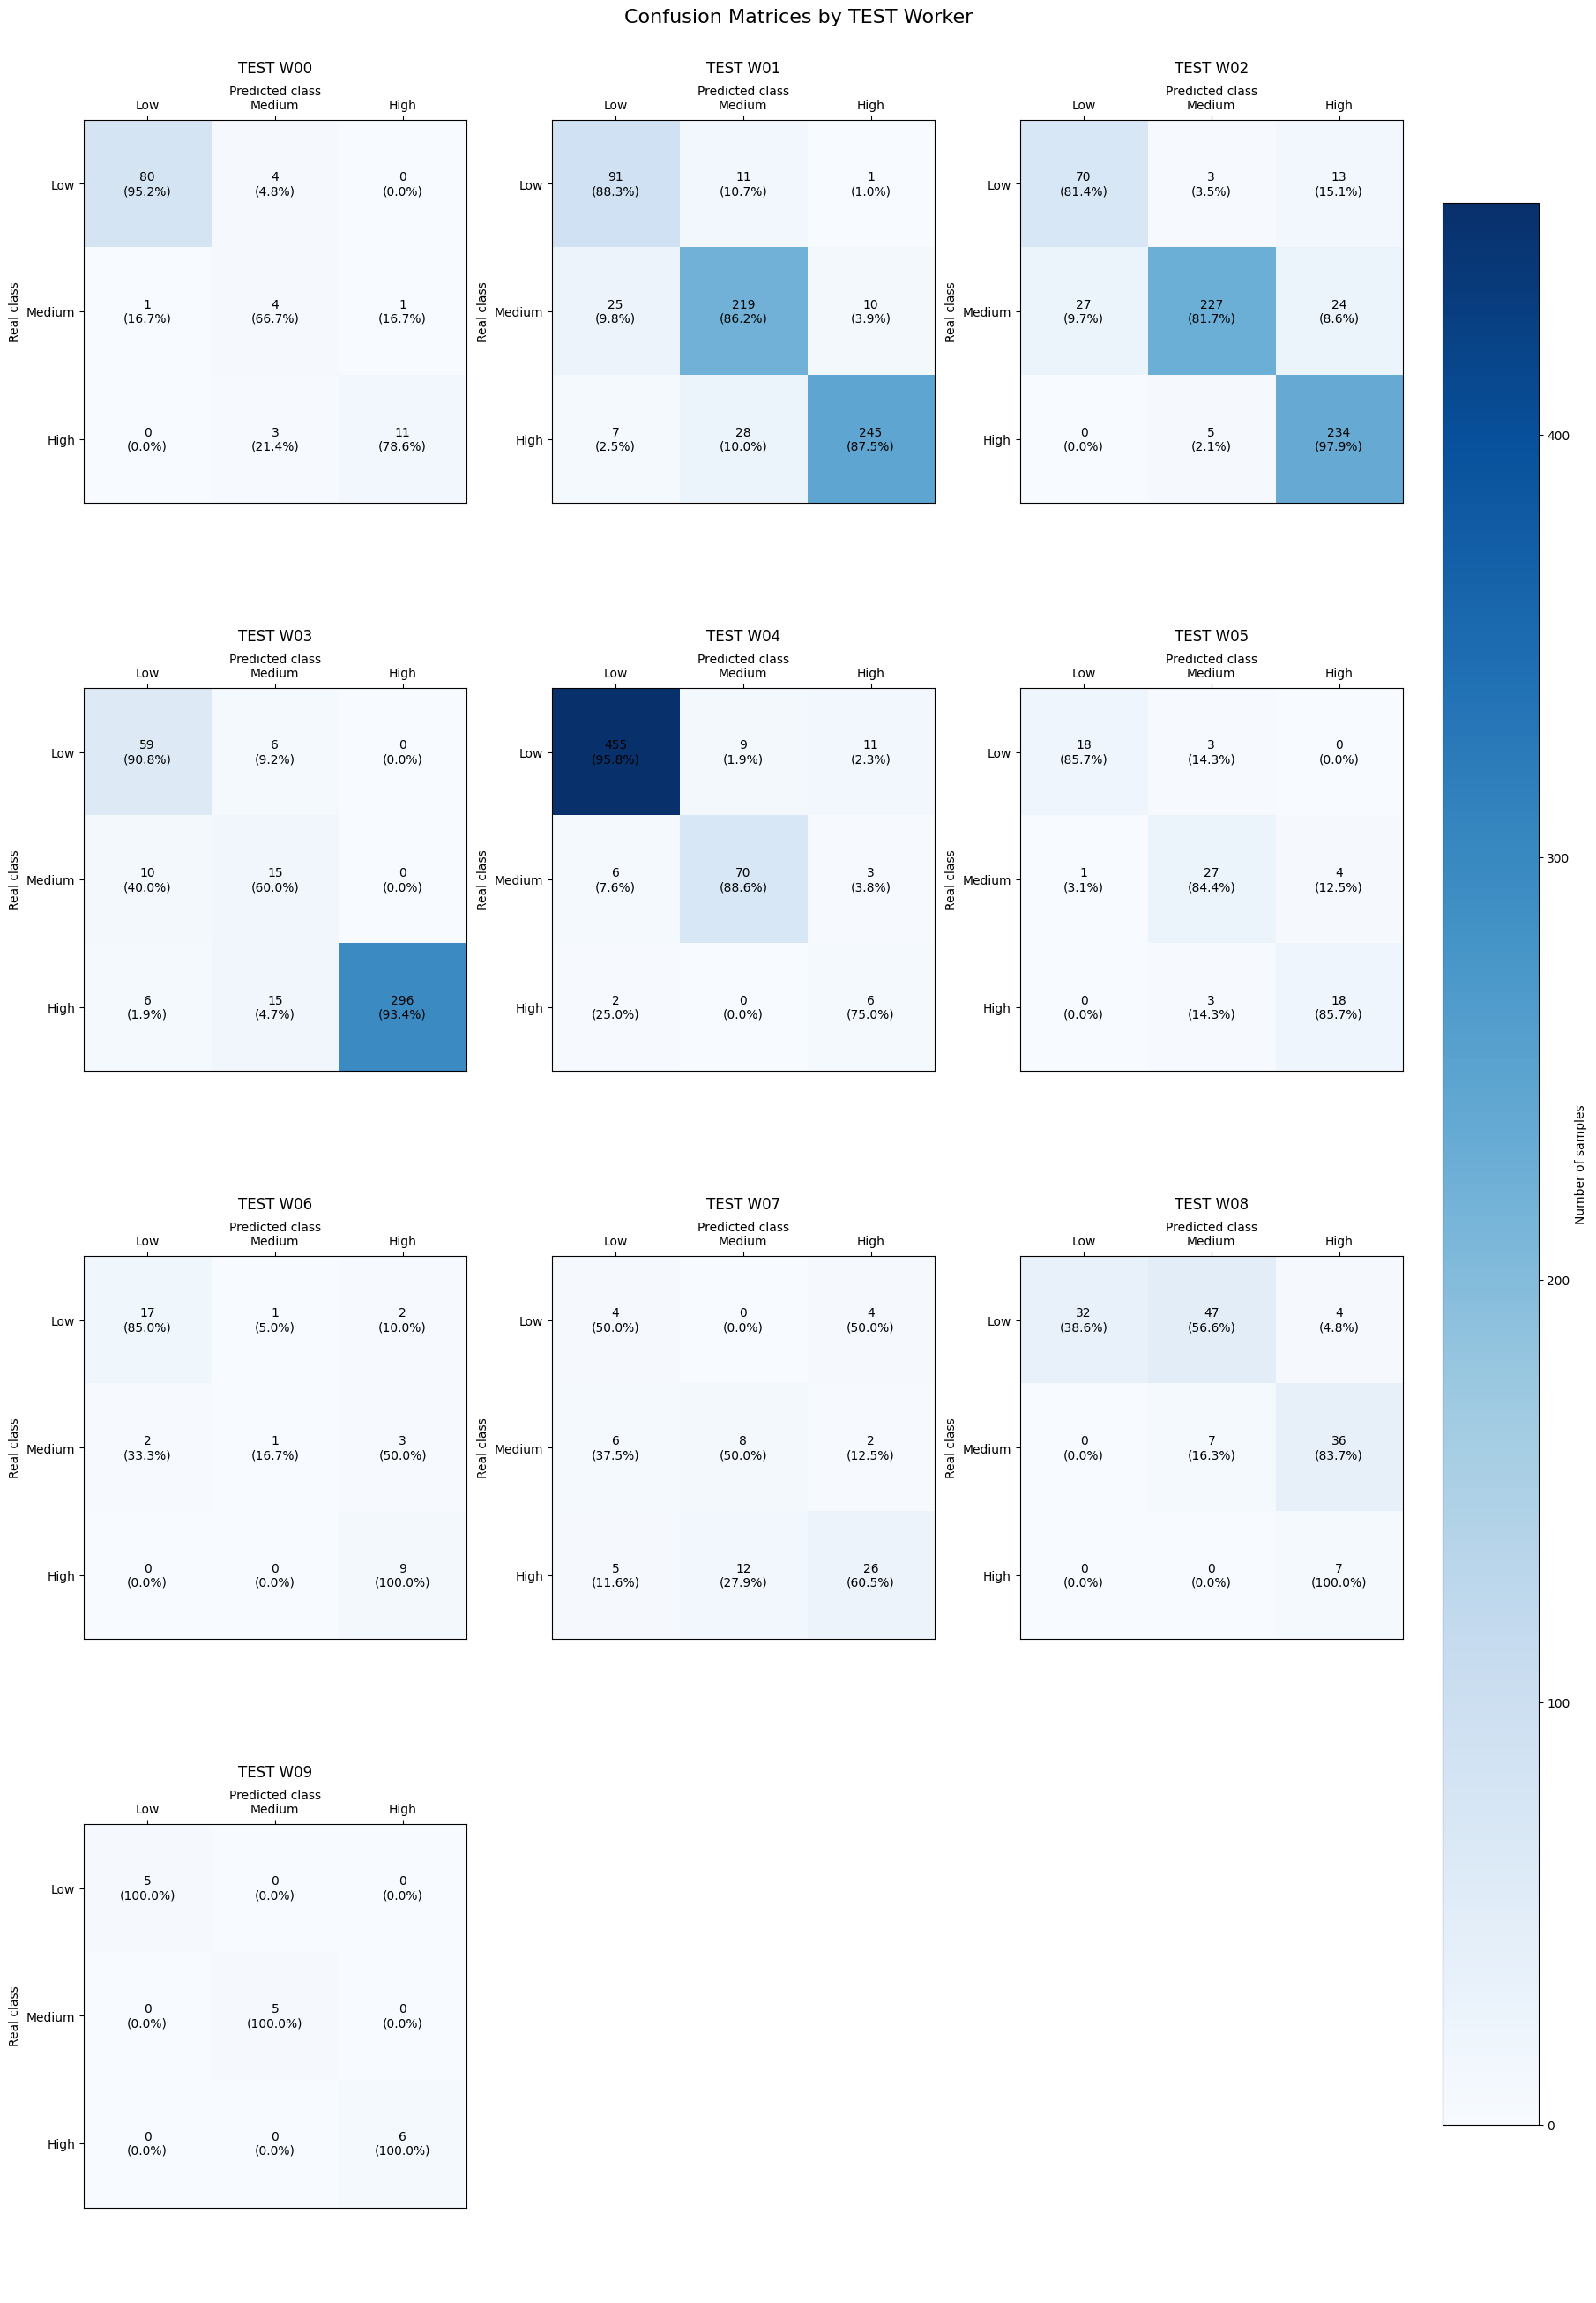
\includegraphics[width=\textwidth,height=\dimexpr\textheight-\pagetotal-4\baselineskip\relax,keepaspectratio]{ch4/assets/confucionsvm.png}
\captionof{figure}{Matrizes de confusão do SVM por trabalhador de teste.}
\label{fig:confusao_svm}
\end{center}

\section{Resultados: Modelo de Regressão Logística}

Os resultados seguintes apresentam o desempenho do modelo de Regressão Logística na validação LOSO com dados do Polar H10. A análise inclui a Tabela~\ref{tab:loso_logistica_detalhado}, que apresenta o desempenho por trabalhador, a Tabela~\ref{tab:classification_report_logistica}, correspondente ao relatório de classificação por classe, e a Tabela~\ref{tab:matriz_confusao_agregada_logistica}, que apresenta a matriz de confusão agregada dos dez folds. A Figura~\ref{fig:confusao_logistica} apresenta as matrizes de confusão individuais para cada trabalhador utilizado como conjunto de teste.

\subsection{Tabela de desempenho da validação LOSO}

A tabela apresenta, para cada trabalhador utilizado como teste, o conjunto de trabalhadores utilizado no treino e as principais métricas de avaliação do modelo.

\begin{table}[H]
\centering
\caption{Validação LOSO do modelo de Regressão Logística.}
\label{tab:loso_logistica_detalhado}
\tiny
\resizebox{\textwidth}{!}{%
\begin{tabular}{l l r r r r r r}
\hline
\textbf{Teste} & \textbf{Treino} & \textbf{Recall LOW} & \textbf{Recall MED} & \textbf{Recall HIGH} & \textbf{Accuracy} & \textbf{Balanced Accuracy} & \textbf{Macro-F1} \\
\hline
W00 & W01--W09 & 0,988095 & 0,500000 & 0,642857 & 0,913462 & 0,710317 & 0,719693 \\
W01 & W00, W02--W09 & 0,883495 & 0,917323 & 0,932143 & 0,918367 & 0,910987 & 0,916154 \\
W02 & W00--W01, W03--W09 & 0,825581 & 0,787770 & 0,974895 & 0,867330 & 0,862749 & 0,868084 \\
W03 & W00--W02, W04--W09 & 0,984615 & 0,600000 & 0,933754 & 0,921376 & 0,839456 & 0,791181 \\
W04 & W00--W03, W05--W09 & 0,842105 & 0,696203 & 0,750000 & 0,820285 & 0,762769 & 0,619439 \\
W05 & W00--W04, W06--W09 & 0,857143 & 0,812500 & 0,761905 & 0,810811 & 0,810516 & 0,815200 \\
W06 & W00--W05, W07--W09 & 0,850000 & 0,833333 & 0,666667 & 0,800000 & 0,783333 & 0,765598 \\
W07 & W00--W06, W08--W09 & 1,000000 & 0,062500 & 0,279070 & 0,313433 & 0,447190 & 0,283677 \\
W08 & W00--W07, W09 & 0,518072 & 0,976744 & 0,000000 & 0,639098 & 0,498272 & 0,437843 \\
W09 & W00--W08 & 1,000000 & 0,400000 & 1,000000 & 0,812500 & 0,800000 & 0,790476 \\
\hline
\textbf{Média} & \textit{Média dos folds} & 0,874911 & 0,658637 & 0,694129 & 0,781666 & 0,742559 & 0,700735 \\
\hline
\end{tabular}%
}
\end{table}

\subsection{Relatório de classificação por classe}

O relatório de classificação por classe apresenta o \textit{support}, o \textit{recall} e a \textit{precision} obtidos para as categorias LOW, MED e HIGH na avaliação LOSO.

\begin{table}[H]
\centering
\caption{Relatório de Classificação por Classe (Classification Report) da Regressão Logística na avaliação LOSO.}
\label{tab:classification_report_logistica}
\begin{tabular}{l c c c}
\hline
\textbf{Classe} & \textbf{Support} & \textbf{Recall} & \textbf{Precision} \\
\hline
Low & 950 & 0,842 & 0,914 \\
Medium & 744 & 0,808 & 0,726 \\
High & 944 & 0,895 & 0,904 \\
\hline
\end{tabular}
\end{table}

\subsection{Matriz de confusão agregada}

A matriz de confusão agregada reúne as previsões dos dez folds. As linhas representam as classes reais e as colunas representam as classes previstas pelo modelo.

\begin{table}[H]
\centering
\caption{Matriz de Confusão Agregada dos Dez Folds da Regressão Logística na avaliação LOSO.}
\label{tab:matriz_confusao_agregada_logistica}
\begin{tabular}{l c c c}
\hline
 & \textbf{Low} & \textbf{Medium} & \textbf{High} \\
\hline
\textbf{Low} & 800 & 146 & 4 \\
\textbf{Medium} & 57 & 601 & 86 \\
\textbf{High} & 18 & 81 & 845 \\
\hline
\end{tabular}
\end{table}

\clearpage
\subsection{Matrizes de confusão por trabalhador}

A figura apresenta as matrizes de confusão individuais obtidas para cada trabalhador utilizado como conjunto de teste.

\begin{center}
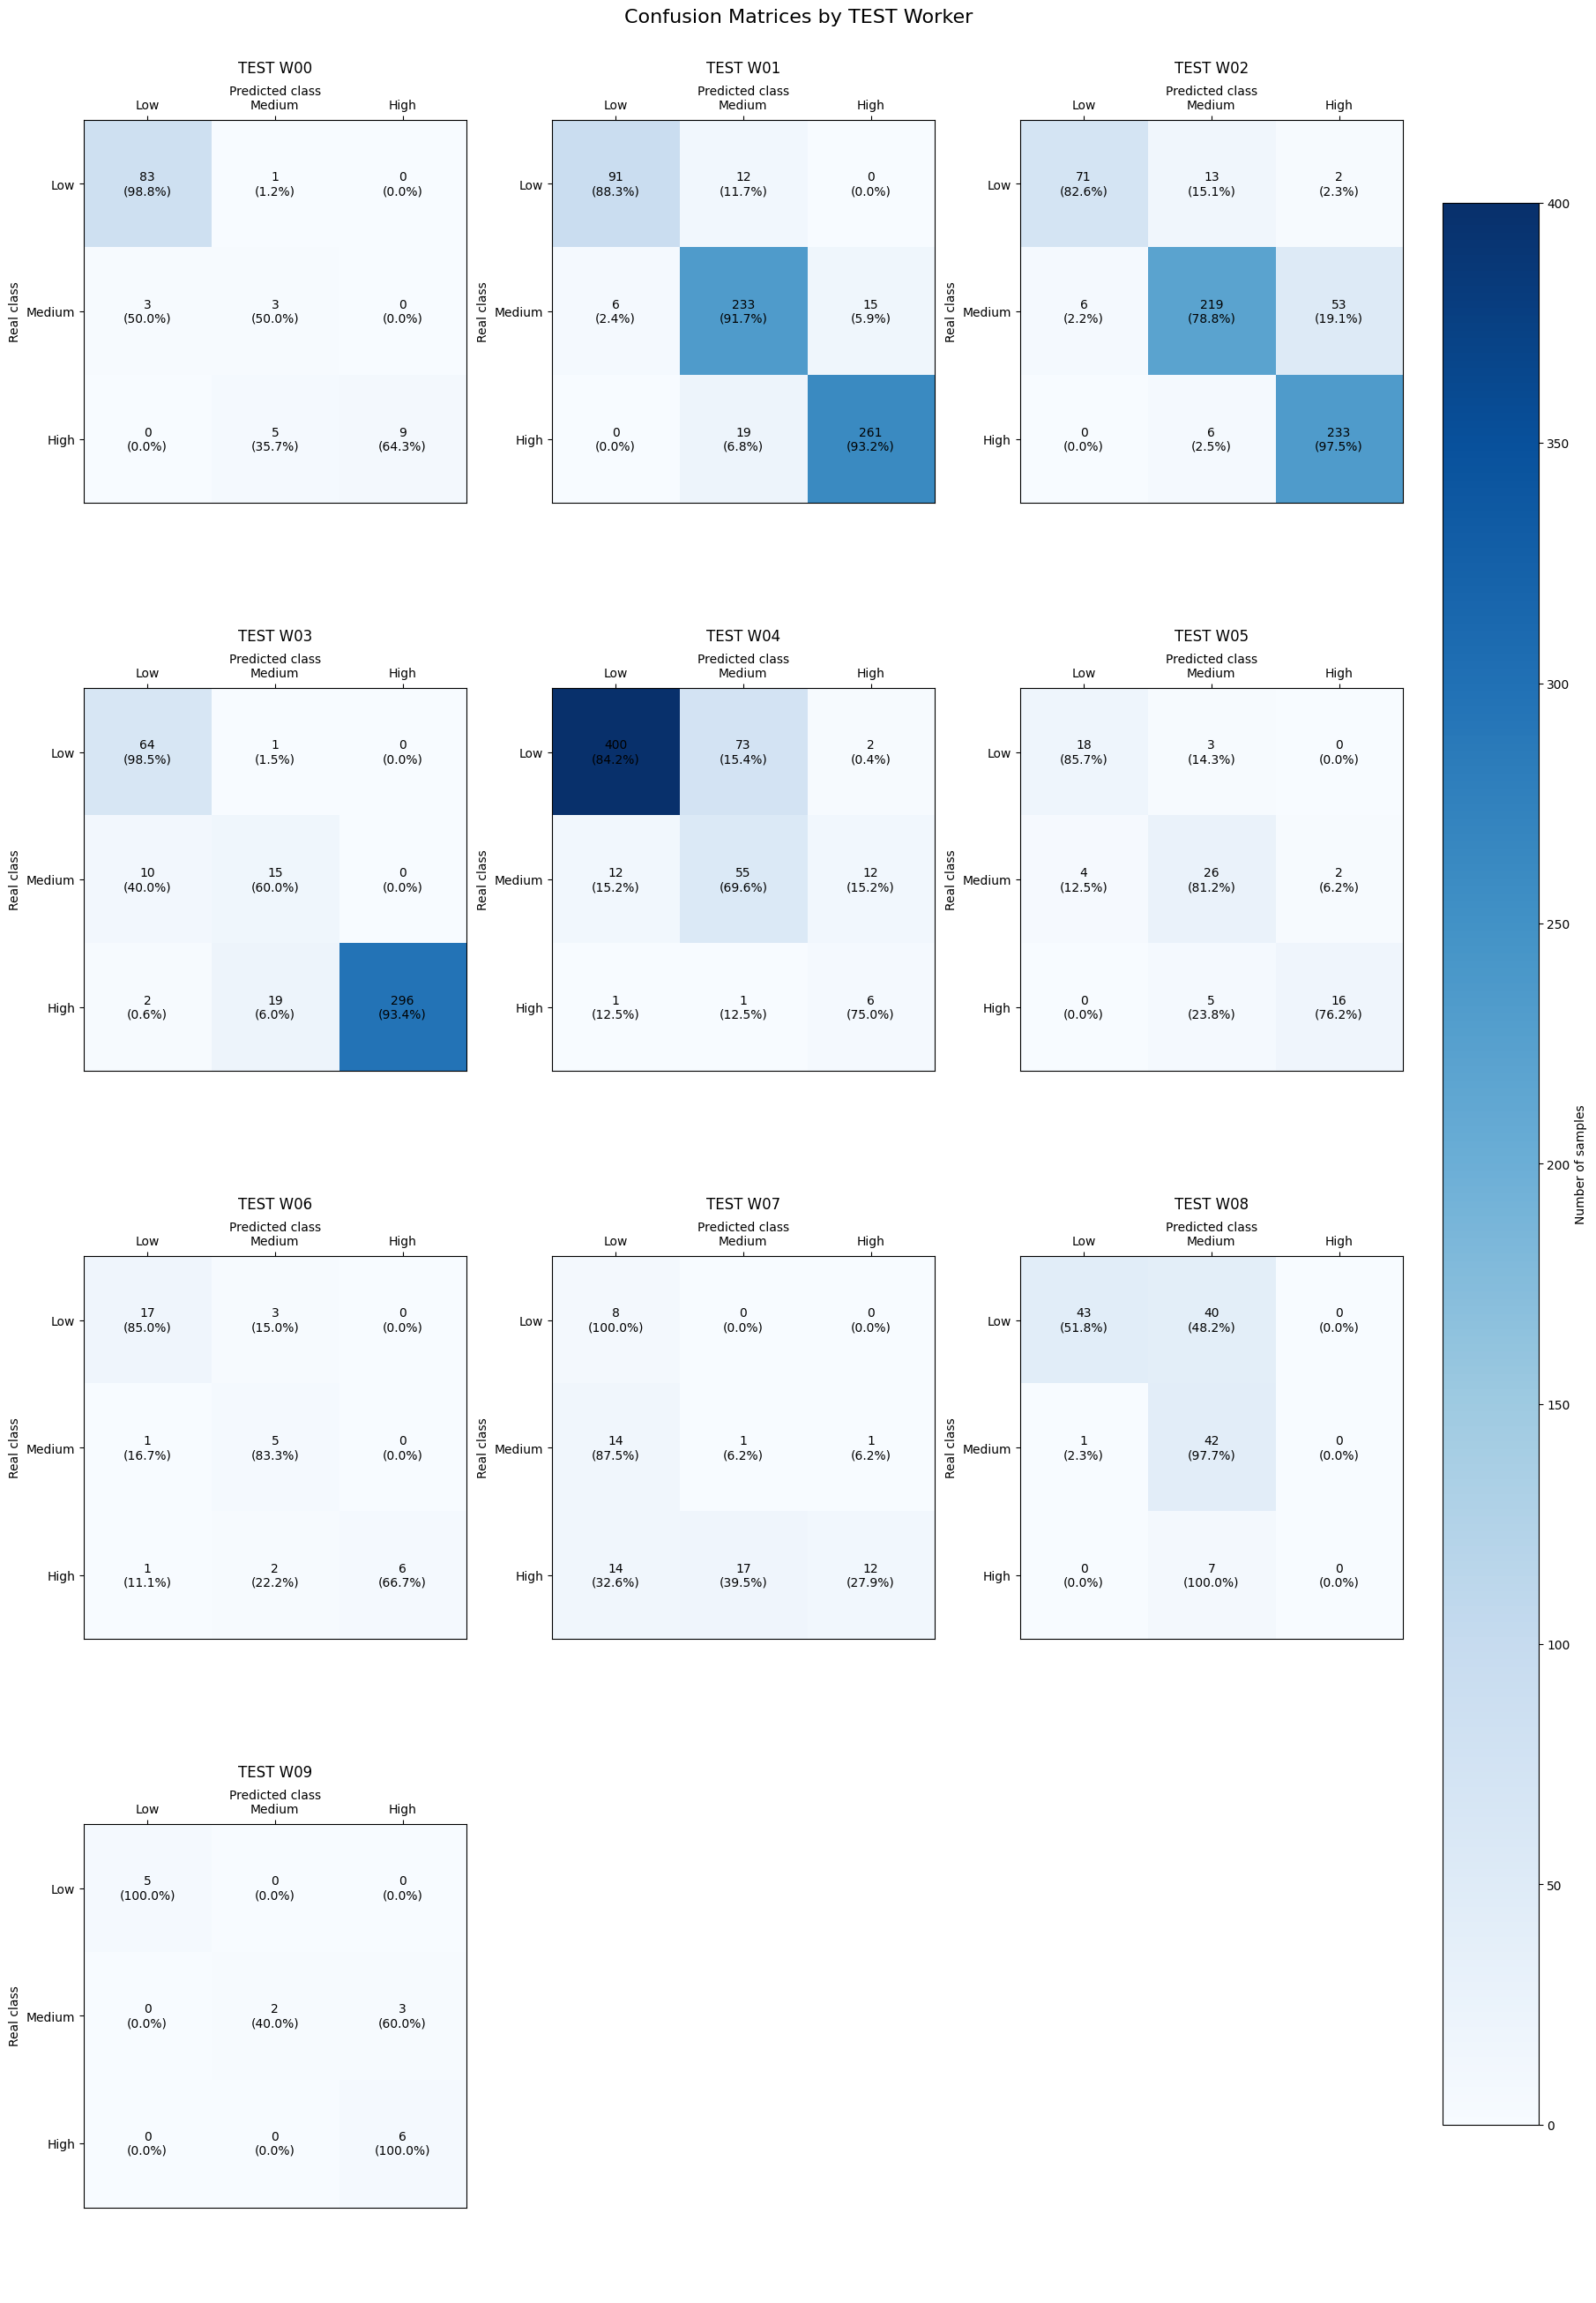
\includegraphics[width=\textwidth,height=\dimexpr\textheight-\pagetotal-4\baselineskip\relax,keepaspectratio]{ch4/assets/confusionlogisticregresion.png}
\captionof{figure}{Matrizes de confusão da Regressão Logística por trabalhador de teste.}
\label{fig:confusao_logistica}
\end{center}

\clearpage
\section{Resultados: Modelo XGBoost}

Os resultados seguintes apresentam, na Figura~\ref{fig:confusao_xgboost}, as matrizes de confusão do modelo XGBoost para os trabalhadores utilizados como conjunto de teste na validação LOSO com dados do Polar H10. As linhas representam as classes reais e as colunas representam as classes previstas pelo modelo.

\subsection{Matrizes de confusão por trabalhador}

A figura apresenta as matrizes de confusão individuais obtidas para cada trabalhador utilizado como conjunto de teste.

\begin{center}
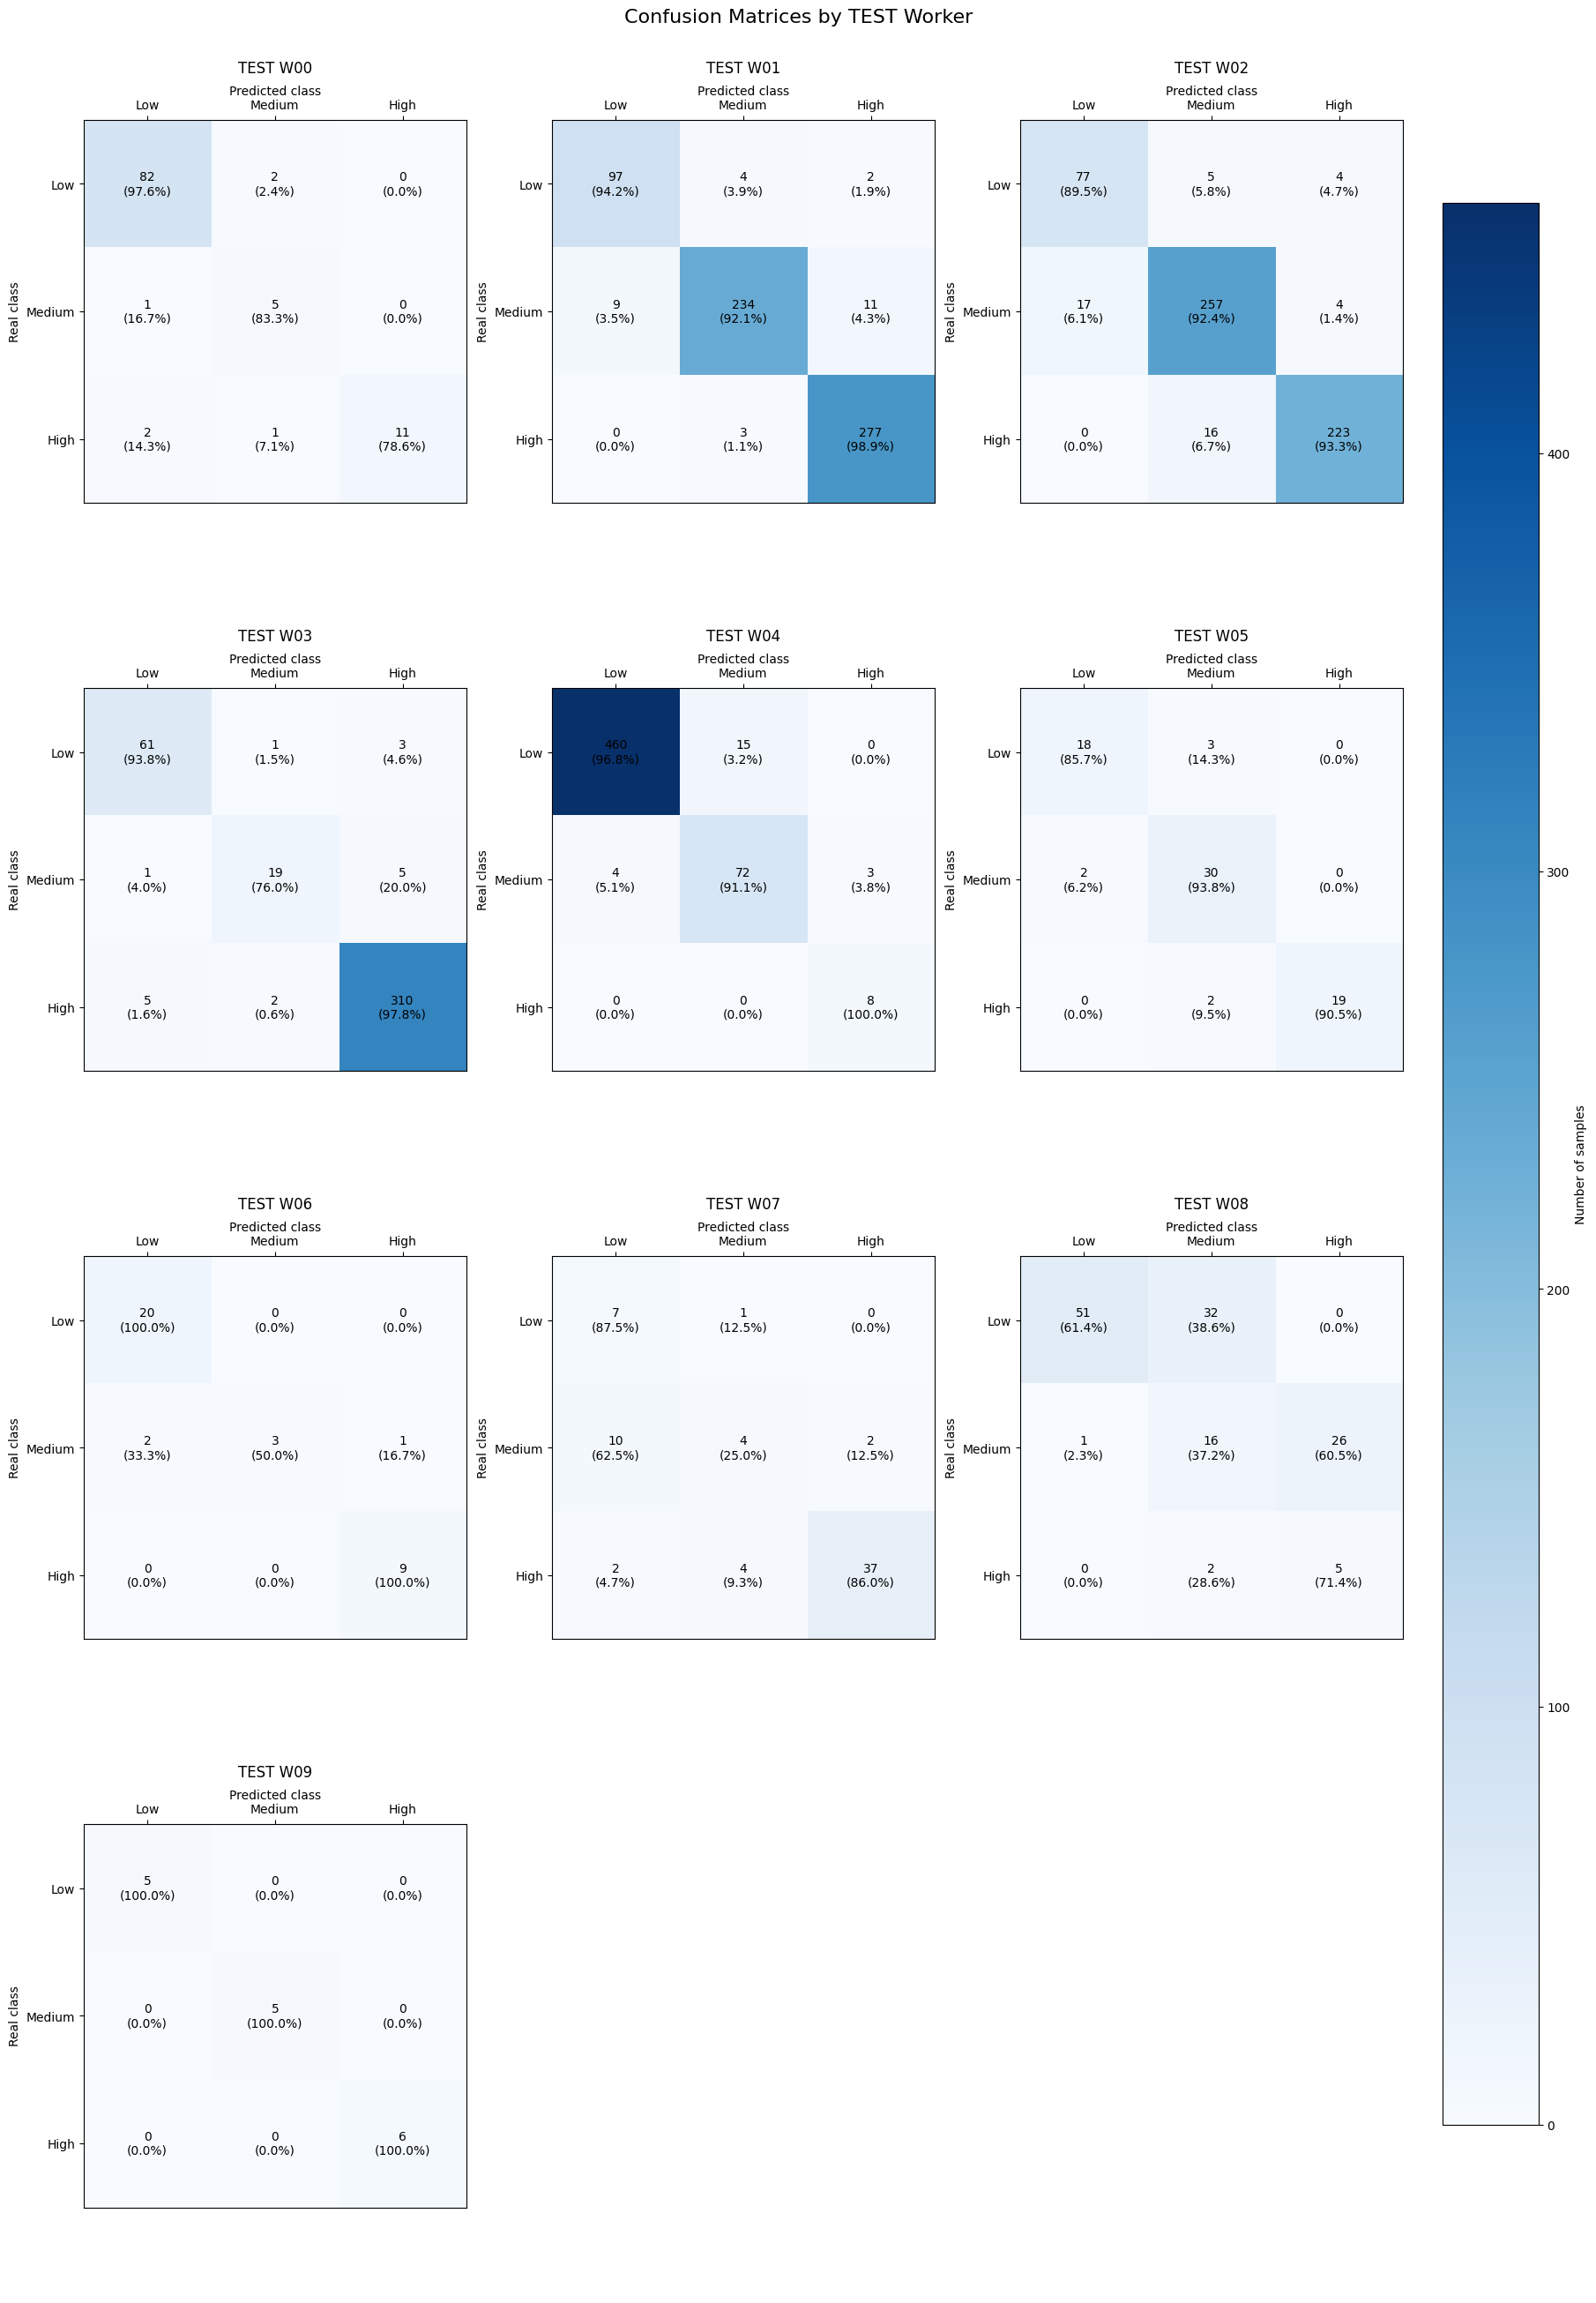
\includegraphics[width=\textwidth,height=\dimexpr\textheight-\pagetotal-4\baselineskip\relax,keepaspectratio]{ch4/assets/confusionxgboost.png}
\captionof{figure}{Matrizes de confusão do XGBoost por trabalhador de teste.}
\label{fig:confusao_xgboost}
\end{center}
